We will now explain how to fill a data file.
First you must specify some basic informations like the dimension of your domain, his name, the problem type...
To define the problem dimension, we use the following keyword:

    \begin{center}
    \fbox{ \begin{minipage}[c]{0.5\textwidth}
    \begin{alltt}
    {\bf{Dimension}}  \textit{2}  or {\bf{Dimension}}  \textit{3}
    \end{alltt}
    \end{minipage}}
    \end{center}


%%%%%%%%%%%%%%%%%%%%%%%%%%%%%%%%%%%%%%%%%%%%%%%%%%%%%%%%%%%%%%%
\section{Problems} \label{pbs}
%%%%%%%%%%%%%%%%%%%%%%%%%%%%%%%%%%%%%%%%%%%%%%%%%%%%%%%%%%%%%%%
You have to define the problem type that you wishes to solve.

    \begin{center}
    \fbox{ \begin{minipage}[c]{0.5\textwidth}
    \begin{alltt}
    {\bf{Pb\textit{\_type}}} \textit{my\_problem}
    \end{alltt}
    \end{minipage}}
    \end{center}

Here are some of the available problems types:
\begin{itemize}
%\item \textbf{Pb\_Hydraulique$\left[\mbox{\_Turbulent}\right]$}
%\item \textbf{Pb\_Thermohydraulique$\left[\mbox{\_Turbulent}\right]$}
%\item \textbf{Pb\_Hydraulique\_Concentration$\left[\mbox{\_Turbulent}\right]$}
\item for incompressible flow: \textbf{Pb\_$\left[\mbox{\textcolor{magenta}{Thermo}}\right]$hydraulique$\left[\mbox{\textcolor{darkblue}{\_Concentration}}\right]\hspace{-0.15cm}\left[\mbox{\textcolor{Greeen}{\_Turbulent}}\right]$},
\item for quasi-compressible flow: \textbf{Pb\_Thermohydraulique$\left[\mbox{\textcolor{Greeen}{\_Turbulent}}\right]$\_QC}, 
%\item for quasi-compressible flow:\\
%    \textbf{Pb\_Thermohydraulique$\left[\mbox{\textcolor{Greeen}{\_Turbulent}}\right]$\_QC$\left[\mbox{\textcolor{mauve}{\_fraction\_massique}}\right]$}, 
\item for solid: \textbf{Pb\_Conduction},
\item you can find all \href{TRUST_Reference_Manual.pdf\#Pbbase}{problem types} in the Reference Manual.
\end{itemize}


where:
\begin{itemize}
\item \textbf{hydraulique}: means that we will solve Navier Stokes equations without energy equation,
\item \textbf{\textcolor{magenta}{Thermo}}: means that we will solve Navier Stokes equations with energy equation,
\item \textbf{\textcolor{darkblue}{Concentration}}: that we will solve multiple constituent transportation equations,
\item \textbf{\textcolor{Greeen}{Turbulent}}: that we will simulate a turbulent flow and specify a turbulent model (RANS or LES),
\item \textbf{Conduction}: resolution of the heat equation,
\item \textbf{QC}: Navier Stokes equations with energy equation for quasi-compressible fluid under low Mach numbers,
%\item \textbf{\textcolor{mauve}{fraction\_massique}}: hydraulic and energy equations are solved and a list of passive scalar equations may be added.
\end{itemize}





%%%%%%%%%%%%%%%%%%%%%%%%%%%%%%%%%%%%%%%%%%%%%%%%%%%%%%%%%%%%%%%
\section{Domain definition}
%%%%%%%%%%%%%%%%%%%%%%%%%%%%%%%%%%%%%%%%%%%%%%%%%%%%%%%%%%%%%%%
To define the domain, you must name. This is done thanks to the following block:

    \begin{center}
    \fbox{ \begin{minipage}[c]{0.5\textwidth}
    \begin{alltt}
    {\bf{Domaine}}  \textit{my\_domain}
    \end{alltt}
    \end{minipage}}
    \end{center}

Then you must add your mesh to your simulation.




%%%%%%%%%%%%%%%%%%%%%%%%%%%%%%%%%%%%%%%%%%%%%%%%%%%%%%%%%%%%%%%
\section{Mesh} \label{Mesh}
%%%%%%%%%%%%%%%%%%%%%%%%%%%%%%%%%%%%%%%%%%%%%%%%%%%%%%%%%%%%%%%

Notice the presence of the tags:
\begin{alltt} 
\textcolor{blue}{\# BEGIN MESH \#}
...
\textcolor{blue}{\# END MESH \#}
\end{alltt}
in the data file of section \ref{data}.
This is necessary for parallel calculation (see section \ref{parallel}).

%%%%%%%%%%%%%%%%%%%%%%%%%%%%%%%%%%%%%%
\subsection{Allowed meshes}
%%%%%%%%%%%%%%%%%%%%%%%%%%%%%%%%%%%%%%
\trust allows:
\begin{itemize}
\item quadrangular or triangular undeformed meshing for 2D cases (Figure \ref{2D_mesh}),
\begin{figure}[h!]
\begin{center}
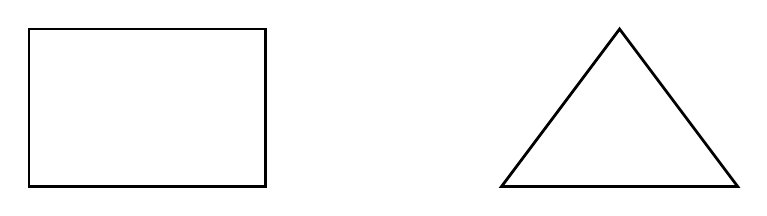
\begin{tikzpicture}[scale=2, line width=1pt]
\coordinate (A) at (0,0) ;
\coordinate (B) at (1.5,0) ;
\coordinate (C) at (1.5,1) ;
\coordinate (D) at (0,1) ;
\draw[black] (A) -- (B) -- (C) -- (D) -- cycle ;
\coordinate (E) at (3,0) ;
\coordinate (F) at (4.5,0) ;
\coordinate (G) at (3.75,1) ;
\draw[black] (E) -- (F) -- (G) -- cycle ;
\end{tikzpicture}
\caption{2D allowed elements}
\label{2D_mesh}
\end{center}
\end{figure}

\item hexahedral or tetrahedral undeformed meshing for 3D cases (Figure \ref{3D_mesh}).
\begin{figure}[h!]
\begin{center}
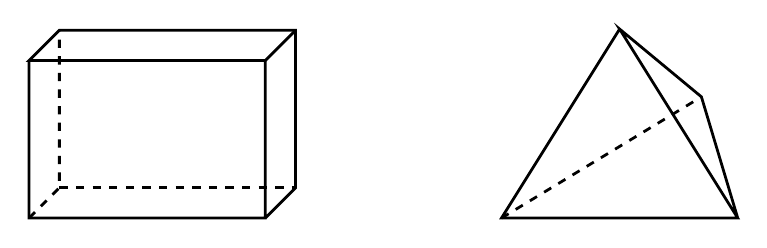
\begin{tikzpicture}[scale=2, line width=1pt]
\coordinate (A) at (0  ,0  ,0) ;
\coordinate (B) at (1.5,0  ,0) ;
\coordinate (C) at (1.5,1  ,0) ;
\coordinate (D) at (0  ,1  ,0) ;
\coordinate (E) at (0  ,0  ,-0.5) ;
\coordinate (F) at (1.5,0  ,-0.5) ;
\coordinate (G) at (1.5,1  ,-0.5) ;
\coordinate (H) at (0  ,1  ,-0.5) ;
\draw (D) -- (A) -- (B) -- (C) -- (D) -- (H) -- (G) -- (F) -- (B);
\draw (C) -- (G);
\draw [dashed] (A) -- (E) -- (H);
\draw [dashed] (E) -- (F);
\coordinate (I) at (3   ,0  ,0) ;
\coordinate (J) at (4.5 ,0  ,0) ;
\coordinate (K) at (3.75,1.2,0) ;
\coordinate (L) at (4   ,0.5,-0.7) ;
\draw[black] (K) -- (I) -- (J) -- (K) -- (L) -- (J) ;
\draw [dashed] (I) -- (L);
\end{tikzpicture}
\caption{3D allowed elements}
\label{3D_mesh}
\end{center}
\end{figure}
\end{itemize}

\textbf{Be carefull} non standard and hybrih meshing are not supported! (cf Figure \ref{hybr})

\begin{figure}[h!]
\begin{center}
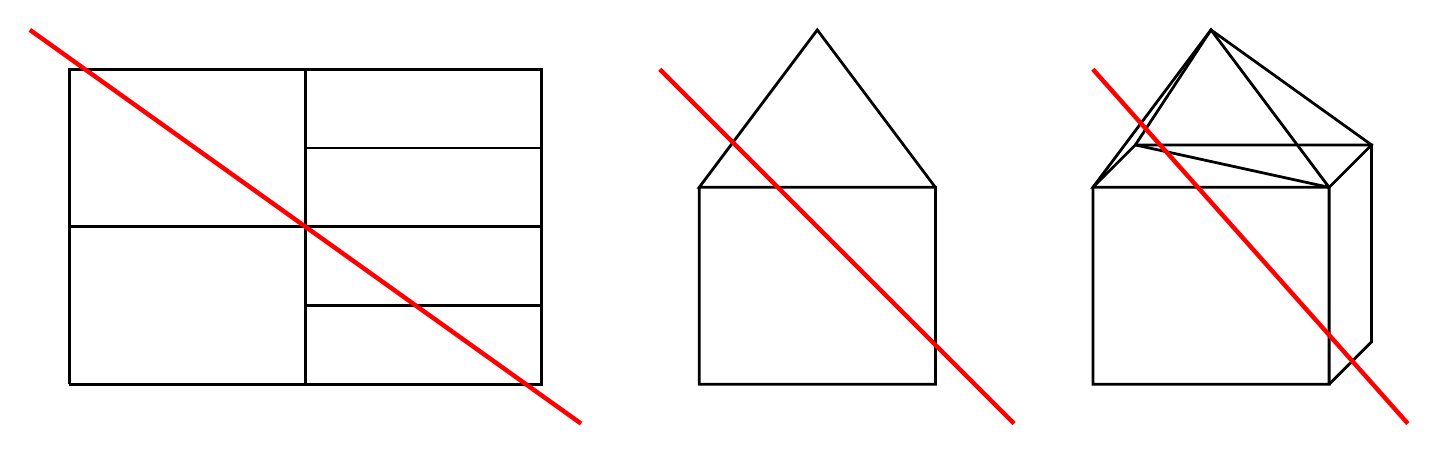
\begin{tikzpicture}[scale=2, line width=1pt]
\coordinate (A1) at (0,0) ;
\coordinate (A2) at (0,1) ;
\coordinate (A3) at (0,2) ;
\coordinate (B1) at (1.5,0  ) ;
\coordinate (B2) at (1.5,0.5) ;
\coordinate (B3) at (1.5,1  ) ;
\coordinate (B4) at (1.5,1.5) ;
\coordinate (B5) at (1.5,2  ) ;
\coordinate (C1) at (3,0  ) ;
\coordinate (C2) at (3,0.5) ;
\coordinate (C3) at (3,1  ) ;
\coordinate (C4) at (3,1.5) ;
\coordinate (C5) at (3,2  ) ;
\draw (A1) -- (C1) -- (C5) -- (A3) -- (A1);
\draw (A2) -- (C3);
\draw (B1) -- (B5);
\draw (B4) -- (C4);
\draw (B2) -- (C2);
\draw [ultra thick,red] (-0.25,2.25) -- (3.25,-0.25) ;

\coordinate (D1) at (4   ,0) ;
\coordinate (D2) at (5.5 ,0) ;
\coordinate (D3) at (5.5 ,1.25) ;
\coordinate (D4) at (4   ,1.25) ;
\coordinate (D5) at (4.75,2.25) ;
\draw (D4) -- (D1) -- (D2) -- (D3) -- (D4) -- (D5) -- (D3);
\draw [ultra thick,red] (3.75,2) -- (6,-0.25) ;

\coordinate (E1) at (6.5 ,0   ,0) ;
\coordinate (E2) at (8   ,0   ,0) ;
\coordinate (E3) at (8   ,1.25,0) ;
\coordinate (E4) at (6.5 ,1.25,0) ;
\coordinate (E5) at (7.25,2.25,0) ;
\coordinate (E6) at (8   ,0   ,-0.7) ;
\coordinate (E7) at (8   ,1.25,-0.7) ;
\coordinate (E8) at (6.5 ,1.25,-0.7) ;
\draw (E4) -- (E1) -- (E2) -- (E3) -- (E4) -- (E5) -- (E3);
\draw (E2) -- (E6) -- (E7) -- (E8) -- (E4);
\draw (E8) -- (E5) -- (E7) -- (E3) -- (E8);
\draw [ultra thick,red] (6.5,2) -- (8.5,-0.25) ;

\end{tikzpicture}
\caption{Prohibited meshes}
\label{hybr}
\end{center}
\end{figure}









%%%%%%%%%%%%%%%%%%%%%%%%%%%%%%%%%%%%%%
\subsection{Import mesh file}
%%%%%%%%%%%%%%%%%%%%%%%%%%%%%%%%%%%%%%
If your mesh was generated with an external tool like \href{http://www.salome-platform.org}{Salom\'e} (open source software), \href{http://resource.ansys.com/Products/Other+Products/ANSYS+ICEM+CFD}{ICEM} (commercial software), \href{http://gmsh.info/}{Gmsh} (open source software, included in \trust package) or \href{http://www-cast3m.cea.fr/}{Cast3M} (CEA software), then you must use one of the following keyword into your data file:

\begin{itemize}
\item \href{TRUST_Reference_Manual.pdf\#readmed}{\textbf{Read\_MED}} for a MED file from \href{http://www.salome-platform.org}{Salom\'e}, \href{http://gmsh.info/}{Gmsh},... ,
\item \href{TRUST_Reference_Manual.pdf\#readfile}{\textbf{Read\_File}} for a binary mesh file from \href{http://resource.ansys.com/Products/Other+Products/ANSYS+ICEM+CFD}{ICEM},
\item for another format, see the \href{TRUST_Reference_Manual.pdf\#read}{\trust Reference Manual}.
\end{itemize}

If you want to learn how to make a mesh with Salom\'e or Gmsh and read it with \trust, you can go to see the exercises of the \trust tutorial: \href{TRUST_tutorial.pdf\#salome}{here} for Salom\'e and \href{TRUST_tutorial.pdf\#gmsh}{here} for Gmsh.




%%%%%%%%%%%%%%%%%%%%%%%%%%%%%%%%%%%%%%
\subsection{Create quickly a mesh}
%%%%%%%%%%%%%%%%%%%%%%%%%%%%%%%%%%%%%%
Here is an example of a simple geometry (of non complex channel type) using the internal tool of \trust:
\begin{center}
\fbox{ \begin{minipage}[c]{0.9\textwidth}
\begin{alltt}
{\bf{Mailler}} \textit{my\_domain}

\{

\hspace{1cm}        \textcolor{blue}{/* Define the domain with one cavity */}

\hspace{1cm}        \textcolor{blue}{/* cavity 1m*2m with 5*22 cells */}

\hspace{1cm}        {\bf{Pave}} \textit{box}

\hspace{1cm}        \{

\hspace{2cm}            {\bf{Origine}} 0. 0.

\hspace{2cm}            {\bf{Longueurs}} 1 2

\hspace{2cm}            \textcolor{blue}{/* Cartesian grid */}

\hspace{2cm}            {\bf{Nombre\_de\_Noeuds}} 6 23

\hspace{2cm}            \textcolor{blue}{/* Uniform mesh */}

\hspace{2cm}            {\bf{Facteurs}} 1. 1.

\hspace{1cm}        \}

\hspace{1cm}        \{

\hspace{2cm}            \textcolor{blue}{/* Definition and names of boundary conditions */}

\hspace{2cm}            {\bf{bord}} \textit{Inlet}   \hspace{0.25cm} X = 0.  0. <= Y <= 2.

\hspace{2cm}            {\bf{bord}} \textit{Outlet}  \hspace{0.05cm} X = 1.  0. <= Y <= 2.

\hspace{2cm}            {\bf{bord}} \textit{Upper}   \hspace{0.25cm} Y = 2.  0. <= X <= 1.

\hspace{2cm}            {\bf{bord}} \textit{Lower}   \hspace{0.25cm} Y = 0.  0. <= X <= 1.

\hspace{1cm}        \}

\}
\end{alltt}
\end{minipage}}
\end{center}

To use this mesh in your data file, you just have to add the previous block in your data file or save it in a file named for example "\textit{my\_mesh.geo}" and add the line:\\
\begin{center}
\fbox{ \begin{minipage}[c]{0.5\textwidth}
\begin{alltt}
{\bf{Read\_file}} \textit{my\_mesh.geo} \textcolor{red}{{\bf{;}}}
\end{alltt}
\end{minipage}}
\end{center}

\underline{Do not forget the semi-colonn at the end of the line!}\\




%%%%%%%%%%%%%%%%%%%%%%%%%%%%%%%%%%%%%%
\subsection{Transform mesh within data file}
%%%%%%%%%%%%%%%%%%%%%%%%%%%%%%%%%%%%%%
You can also made transformations on your mesh after the \textbf{"Mailler"} or \textbf{"Read\_*"} command, using the following keywords:
\begin{itemize}
\item \href{TRUST_Reference_Manual.pdf\#triangulate}{\textbf{Trianguler}} to triangulate your 2D cells and create an unstructured mesh.
\item \href{TRUST_Reference_Manual.pdf\#tetraedriser}{\textbf{Tetraedriser}} to tetrahedralise 3D cells and create an unstructured mesh.
\item \href{TRUST_Reference_Manual.pdf\#raffineranisotrope}{\textbf{Raffiner\_anisotrope}}/\href{TRUST_Reference_Manual.pdf\#raffinerisotrope}{\textbf{Raffiner\_isotrope}} to triangulate/tetrahedralise elements of an untructured mesh.
\item \href{TRUST_Reference_Manual.pdf\#extrudebord}{\textbf{ExtrudeBord}} to generate an extruded mesh from a boundary of a tetrahedral or an hexahedral mesh. \Note that ExtrudeBord in VEF generates 3 or 14 tetrahedra from extruded prisms.
\Note that ExtrudeBord in VEF generates 3 or 14 tetrahedra from extruded prisms.
\item \href{TRUST_Reference_Manual.pdf\#regroupebord}{\textbf{RegroupeBord}} to build a new boundary with several boundaries of the domain.
\item \href{TRUST_Reference_Manual.pdf\#transformer}{\textbf{Transformer}} to transform the coordinates of the geometry.
\item for other commands, see the section \href{TRUST_Reference_Manual.pdf\#interprete}{interprete} of the \trust Reference Manual.
\end{itemize}

\Note that theses mesh modifications work on all mesh type (i.e. also for \textbf{*.geo} or \textbf{*.bin} or \textbf{*.med} files).



%%%%%%%%%%%%%%%%%%%%%%%%%%%%%%%%%%%%%%
\subsection{Test your mesh}
%%%%%%%%%%%%%%%%%%%%%%%%%%%%%%%%%%%%%%
The keyword \href{TRUST_Reference_Manual.pdf\#discretiserdomaine}{\textbf{Discretiser\_domaine}} is useful to discretize the domain (faces will be created) without defining a problem.
Indeed, you can create a minimal data file, post-process your mesh in lata format (for example) and visualize it with VisIt. \\

\Note that you must name all the boundaries!\\

Here is an example of this kind of data file:

\begin{center}
\fbox{ \begin{minipage}[c]{0.8\textwidth}
\begin{center}
\textbf{my\_data\_file.data}
\end{center}
\end{minipage}}
\fbox{ \begin{minipage}[c]{0.8\textwidth}
\begin{alltt}
{\bf{dimension 3}}

{\bf{Domaine}} \textit{my\_domain}

{\bf{Mailler}} \textit{my\_domain}

\{

\hspace{1cm}    {\bf{Pave}} \textit{box}

\hspace{1cm}    \{

\hspace{2cm}        {\bf{Origine}} 0. 0. 0.

\hspace{2cm}        {\bf{Longueurs}} 1 2 1

\hspace{2cm}        {\bf{Nombre\_de\_Noeuds}} 6 23 6

\hspace{2cm}        {\bf{Facteurs}} 1. 1. 1.

\hspace{1cm}    \}

\hspace{1cm}    \{

\hspace{2cm}        {\bf{bord}} \textit{Inlet}  \hspace{0.25cm} X = 0. 0. <= Y <= 2.  0. <= Z <= 1.

\hspace{2cm}        {\bf{bord}} \textit{Outlet} \hspace{0.05cm} X = 1.  0. <= Y <= 2.  0. <= Z <= 1.

\hspace{2cm}        {\bf{bord}} \textit{Upper}  \hspace{0.25cm} Y = 2.  0. <= X <= 1.  0. <= Z <= 1.

\hspace{2cm}        {\bf{bord}} \textit{Lower}  \hspace{0.25cm} Y = 0. 0. <= X <= 1.  0. <= Z <= 1.

\hspace{2cm}        {\bf{bord}} \textit{Front}  \hspace{0.25cm} Z = 0. 0. <= X <= 1.  0. <= Y <= 2.

\hspace{2cm}        {\bf{bord}} \textit{Back}   \hspace{0.45cm} Z = 1. 0. <= X <= 1.  0. <= Y <= 2.

\hspace{1cm}    \}

\}

{\bf{discretiser\_domaine}} \textit{my\_domain}

{\bf{postraiter\_domaine}} \{ {\bf{domaine}} \textit{my\_domain} {\bf{format lata}} \}

{\bf{End}}
    \end{alltt}
\end{minipage}}
\end{center}

To use it, launch in a bash terminal:
\begin{verbatim}
# if not already done
> source $my_path_to_TRUST_installation/env_TRUST.sh
# then
> trust my_data_file
> visit -o my_data_file.lata &
\end{verbatim}

To see how to use VisIt, go to see the first tutorial exercise: \href{TRUST_tutorial.pdf\#exo1}{Obstacle}.\\

If you want to learn how to make a mesh with Salom\'e or Gmsh and read it with \trust, you can go to see the exercises of the \trust tutorial: \href{TRUST_tutorial.pdf\#salome}{here} for Salom\'e and \href{TRUST_tutorial.pdf\#gmsh}{here} for Gmsh.



%%%%%%%%%%%%%%%%%%%%%%%%%%%%%%%%%%%%%%%%%%%%%%%%%%%%%%%%%%%%%%%
\section{Parallel calculation}
%%%%%%%%%%%%%%%%%%%%%%%%%%%%%%%%%%%%%%%%%%%%%%%%%%%%%%%%%%%%%%%
For parallel calculation, we need two additional blocks.


%%%%%%%%%%%%%%%%%%%%%%%%%%%%%%%%%%%%%%
\subsection{Partitioning}
%%%%%%%%%%%%%%%%%%%%%%%%%%%%%%%%%%%%%%


%%%%%%%%%%%%%%%%%%%%%%%%%%%%%%%%%%%%%%
\subsection{Read the sub-domains}
%%%%%%%%%%%%%%%%%%%%%%%%%%%%%%%%%%%%%%



%%%%%%%%%%%%%%%%%%%%%%%%%%%%%%%%%%%%%%%%%%%%%%%%%%%%%%%%%%%%%%%
\section{Discretization}
%%%%%%%%%%%%%%%%%%%%%%%%%%%%%%%%%%%%%%%%%%%%%%%%%%%%%%%%%%%%%%%
You have to specify the discretization type which can be \href{TRUST_Reference_Manual.pdf\#vdf}{\textbf{VDF}}, \href{TRUST_Reference_Manual.pdf\#ef}{\textbf{EF}} or \href{TRUST_Reference_Manual.pdf\#vefprep1b}{\textbf{VEFPreP1B}}.\\

In \textbf{VDF} discretization, the locations of the unknown are drawn in the Figure \ref{fig_VDF}.\\

\begin{figure}[h!]
\begin{center}
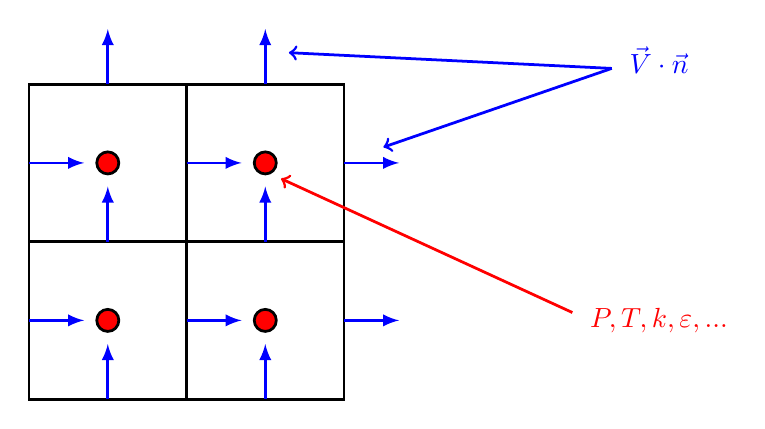
\begin{tikzpicture}[scale=2, line width=1pt]
\coordinate (A) at (0,0) ;
\coordinate (B) at (1,0) ;
\coordinate (C) at (2,0) ;
\coordinate (D) at (2,1) ;
\coordinate (E) at (2,2) ;
\coordinate (F) at (1,2) ;
\coordinate (G) at (0,2) ;
\coordinate (H) at (0,1) ;
\draw[black] (A) -- (C) -- (E) -- (G) -- cycle ;
\draw[black] (H) -- (D) ;
\draw[black] (F) -- (B) ;
\draw[black,fill=red] (0.5,0.5) circle (0.07);
\draw[black,fill=red] (1.5,0.5) circle (0.07);
\draw[black,fill=red] (0.5,1.5) circle (0.07);
\draw[black,fill=red] (1.5,1.5) circle (0.07);
\draw[blue] [->] [>=latex] (0.5,0) -- (0.5,0.35);
\draw[blue] [->] [>=latex] (0.5,1) -- (0.5,1.35);
\draw[blue] [->] [>=latex] (0.5,2) -- (0.5,2.35);
\draw[blue] [->] [>=latex] (1.5,0) -- (1.5,0.35);
\draw[blue] [->] [>=latex] (1.5,1) -- (1.5,1.35);
\draw[blue] [->] [>=latex] (1.5,2) -- (1.5,2.35);
\draw[blue] [->] [>=latex] (0,0.5) -- (0.35,0.5);
\draw[blue] [->] [>=latex] (1,0.5) -- (1.35,0.5);
\draw[blue] [->] [>=latex] (2,0.5) -- (2.35,0.5);
\draw[blue] [->] [>=latex] (0,1.5) -- (0.35,1.5);
\draw[blue] [->] [>=latex] (1,1.5) -- (1.35,1.5);
\draw[blue] [->] [>=latex] (2,1.5) -- (2.35,1.5);
\draw[blue] (4,2) node[above]{$\vec{V} \cdot \vec{n}$} ;
\draw[blue] [<-] (1.65,2.2) -- (3.7,2.1);
\draw[blue] [<-] (2.25,1.6) -- (3.7,2.1);
\draw[red] (4,0.5) node {$P, T, k, \varepsilon, ...$} ;
\draw[red] [<-] (1.6,1.4) -- (3.45,0.55);
\end{tikzpicture}
\caption{VDF unknown localisations}
\label{fig_VDF}
\end{center}
\end{figure}

For \textbf{VEFPreP1B}, the locations of the unknown are drawn in the Figure \ref{fig_VEF}.\\

\begin{figure}[h!]
\begin{center}
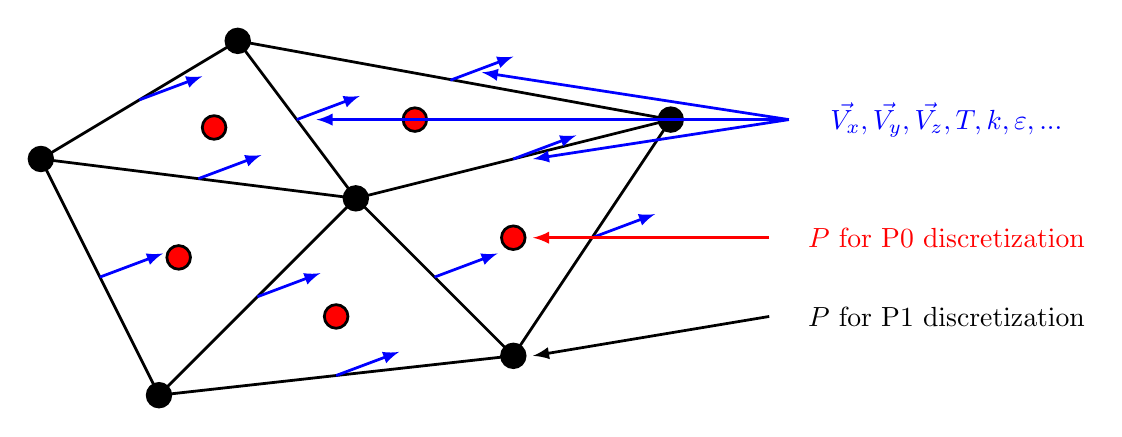
\begin{tikzpicture}[scale=1, line width=1pt]
\coordinate (A) at (1.5,0) ;
\coordinate (B) at (6,0.5) ;
\coordinate (C) at (8,3.5) ;
\coordinate (D) at (2.5,4.5) ;
\coordinate (E) at (0,3) ;
\coordinate (F) at (4,2.5) ;
\draw[black] (A) -- (B) -- (C) -- (D) -- (E) -- (A) -- (F) -- (B);
\draw[black] (C) -- (F) -- (D);
\draw[black] (E) -- (F);
\draw[black,fill=black] (A) circle (0.15);
\draw[black,fill=black] (B) circle (0.15);
\draw[black,fill=black] (C) circle (0.15);
\draw[black,fill=black] (D) circle (0.15);
\draw[black,fill=black] (E) circle (0.15);
\draw[black,fill=black] (F) circle (0.15);
\draw[black,fill=red] (3.75,1) circle (0.15);
\draw[black,fill=red] (6,2) circle (0.15);
\draw[black,fill=red] (4.75,3.5) circle (0.15);
\draw[black,fill=red] (2.2,3.4) circle (0.15);
\draw[black,fill=red] (1.75,1.75) circle (0.15);
\begin{scope}[xshift=5cm, yshift=1.5cm]
\draw[blue] [->] [>=latex] (0,0) -- (0.8,0.3);
\end{scope}
\begin{scope}[xshift=7cm, yshift=2cm]
\draw[blue] [->] [>=latex] (0,0) -- (0.8,0.3);
\end{scope}
\begin{scope}[xshift=5.2cm, yshift=4cm]
\draw[blue] [->] [>=latex] (0,0) -- (0.8,0.3);
\end{scope}
\begin{scope}[xshift=1.25cm, yshift=3.75cm]
\draw[blue] [->] [>=latex] (0,0) -- (0.8,0.3);
\end{scope}
\begin{scope}[xshift=0.75cm, yshift=1.5cm]
\draw[blue] [->] [>=latex] (0,0) -- (0.8,0.3);
\end{scope}
\begin{scope}[xshift=2.75cm, yshift=1.25cm]
\draw[blue] [->] [>=latex] (0,0) -- (0.8,0.3);
\end{scope}
\begin{scope}[xshift=3.75cm, yshift=0.25cm]
\draw[blue] [->] [>=latex] (0,0) -- (0.8,0.3);
\end{scope}
\begin{scope}[xshift=6cm, yshift=3cm]
\draw[blue] [->] [>=latex] (0,0) -- (0.8,0.3);
\end{scope}
\begin{scope}[xshift=3.25cm, yshift=3.5cm]
\draw[blue] [->] [>=latex] (0,0) -- (0.8,0.3);
\end{scope}
\begin{scope}[xshift=2cm, yshift=2.75cm]
\draw[blue] [->] [>=latex] (0,0) -- (0.8,0.3);
\end{scope}
\draw[blue] (11.5,3.5) node {$\vec{V_x}, \vec{V_y}, \vec{V_z}, T, k, \varepsilon, ...$} ;
\draw[blue] [->] [>=latex] (9.5,3.5) -- (5.6,4.1);
\draw[blue] [->] [>=latex] (9.5,3.5) -- (3.5,3.5);
\draw[blue] [->] [>=latex] (9.5,3.5) -- (6.25,3);
\draw[red] (11.5,2) node {$P$ for P0 discretization} ;
\draw[red] [->] [>=latex] (9.25,2) -- (6.25,2);
\draw[black] (11.5,1) node {$P$ for P1 discretization} ;
\draw[black] [->] [>=latex] (9.25,1) -- (6.25,0.5);
\end{tikzpicture}
\caption{VEF unknown localisations in 2D}
\label{fig_VEF}
\end{center}
\end{figure}

In 3D for the pressure, we can also use the P0+P1+Pa discretization for flow with a strong source term and a low velocity field.
In this case P0+P1 pressure gradient has trouble to match the source term so we use P0+P1+Pa discretization (cf Figure \ref{fig_VEF_pressure_loc}).

\begin{figure}[h!]
\begin{center}
\begin{tikzpicture}[scale=1, line width=1pt]
\coordinate (A) at (0.5,1) ;
\coordinate (B) at (3,0.5) ;
\coordinate (C) at (4,2.5) ;
\coordinate (D) at (2,4) ;
\draw[black] (B) -- (C) -- (D) -- (A) -- (B) -- (D);
\draw[black,dashed] (A) -- (C);
\draw[black,fill=black] (A) circle (0.15);
\draw[black,fill=black] (B) circle (0.15);
\draw[black,fill=black] (C) circle (0.15);
\draw[black,fill=black] (D) circle (0.15);
\draw[black,fill=Greeen] (1.75,0.75) circle (0.15);
\draw[black,fill=Greeen] (3.5,1.5) circle (0.15);
\draw[black,fill=Greeen] (3,3.25) circle (0.15);
\draw[black,fill=Greeen] (1.25,2.5) circle (0.15);
\draw[black,fill=Greeen] (2.25,1.75) circle (0.15);
\draw[black,fill=Greeen] (2.5,2.25) circle (0.15);
\draw[black,fill=red] (2.2,2) circle (0.15);
\draw[black] (10,3) node {$P$ for P1 discretization} ;
\draw[black] [->] [>=latex] (7.75,3) -- (2.2,4);
\draw[black] [->] [>=latex] (7.75,3) -- (4.2,2.5);
\draw[red] (10,2) node {$P$ for P0 discretization} ;
\draw[red] [->] [>=latex] (7.75,2) -- (2.5,2);
\draw[Greeen] (10,1) node {$P$ for Pa discretization} ;
\draw[Greeen] [->] [>=latex] (7.75,1) -- (3.7,1.5);
\draw[Greeen] [->] [>=latex] (7.75,1) -- (2,0.75);
\end{tikzpicture}
\caption{VEF pressure localisation in 3D}
\label{fig_VEF_pressure_loc}
\end{center}
\end{figure}

To specify the wanted discretization, you have to add the following block to your data file:

    \begin{center}
    \fbox{ \begin{minipage}[c]{0.5\textwidth}
    \begin{alltt}
    \textit{{\bf{Discretization\_type}} my\_discretization}

    [{\bf{Read }} \textit{my\_discretization \{ ... \}}]
    \end{alltt}
    \end{minipage}}
    \end{center}

You can add parameters to your discretization with the optional keyword \href{TRUST_Reference_Manual.pdf\#read}{\textbf{Read}} (see \href{TRUST_Reference_Manual.pdf\#vefprep1b}{\textbf{VEFPreP1B discretization}}).

On the \href{http://www-trio-u.cea.fr/scripts/home/publigen/content/templates/show.asp?L=EN&P=55&vTicker=alleza&ITEMID=3}{TRUST website}, you can find information about:
\begin{itemize}
\item \textbf{VDF} discretization in the \href{http://www-trio-u.cea.fr/home/liblocal/docs/Theses/these_chatelain_2004.pdf}{PhD thesis of A. Chatelain},
\item \textbf{VEFPreP1B} discretization (Crouzet-Raviart elements) in the \href{http://www-trio-u.cea.fr/home/liblocal/docs/Theses/these_fortin_2006.pdf}{PhD thesis of T. Fortin} and \href{http://www-trio-u.cea.fr/home/liblocal/docs/Theses/These_Heib_2003.pdf}{PhD thesis of S. Heib}.
\end{itemize}


%%%%%%%%%%%%%%%%%%%%%%%%%%%%%%%%%%%%%%%%%%%%%%%%%%%%%%%%%%%%%%%
\section{Time schemes}
%%%%%%%%%%%%%%%%%%%%%%%%%%%%%%%%%%%%%%%%%%%%%%%%%%%%%%%%%%%%%%%
Now you can choose your time scheme to solve your problem. For this you must
specify the time scheme type wanted and give it a name. 
then you have to specify its parameters by filling the associated \textbf{"Read"} block.

    \begin{center}
    \fbox{ \begin{minipage}[c]{0.5\textwidth}
    \begin{alltt}
    {\bf{\textit{Scheme\_type}}} \textit{my\_time\_scheme}

    {\bf{Read}} \textit{my\_time\_scheme} \{ ... \}
    \end{alltt}
    \end{minipage}}
    \end{center}

%%%%%%%%%%%%%%%%%%%%%%%%%%%%%%%%%%%%%%
\subsection{Some available time schemes}
%%%%%%%%%%%%%%%%%%%%%%%%%%%%%%%%%%%%%%
%Here are some \href[page=DOCLINK_TIME SCHEMES]{TRUST_Reference_Manual.pdf}{available types of explicit schemes}:
Here are some available types of explicit schemes:
\begin{itemize}
\item \href{TRUST_Reference_Manual.pdf\#eulerscheme}{\textbf{Scheme\_Euler\_explicit}},
\item \href{TRUST_Reference_Manual.pdf\#schemaadamsbashforthorder2}{\textbf{Schema\_Adams\_Bashforth\_order\_2}},
%\item \textbf{Schema\_Adams\_Bashforth\_order\_3}
%\item \textbf{Runge\_Kutta\_Rationnel\_ordre\_2}
\item \href{TRUST_Reference_Manual.pdf\#rungekuttaordre3}{\textbf{Runge\_Kutta\_ordre\_3}},
%\item \textbf{Runge\_Kutta\_ordre\_4\_D3P}
%\item \textbf{Schema\_Predictor\_Corrector}
%\item \textbf{Sch\_CN\_iteratif}
%\item \textbf{Sch\_CN\_EX\_iteratif}
%\item \textbf{Schema\_Phase\_Field}
%\item \textbf{RK3\_FT}
\end{itemize}

%And also some \href[page=DOCLINK_TIME SCHEMES]{TRUST_Reference_Manual.pdf}{available types of implicit schemes}:
And also some available types of implicit schemes:
\begin{itemize}
\item \href{TRUST_Reference_Manual.pdf\#schemaeulerimplicite}{\textbf{Scheme\_Euler\_implicit}},
%\item \textbf{Schema\_Adams\_Moulton\_order\_2}
\item \href{TRUST_Reference_Manual.pdf\#schemaadamsmoultonorder3}{\textbf{Schema\_Adams\_Moulton\_order\_3}}.
%\item \textbf{Schema\_Backward\_Differentiation\_order\_2}
%\item \textbf{Schema\_Backward\_Differentiation\_order\_3}
\end{itemize}

For other scheme, see \href{TRUST_Reference_Manual.pdf\#schematempsbase}{this section} of the Reference Manual.\\

\Note that you can use semi-implicit schemes activating the \textbf{diffusion\_implicite} keyword in your explicit time scheme.



%%%%%%%%%%%%%%%%%%%%%%%%%%%%%%%%%%%%%%
\subsection{Calculation stopping condition}
%%%%%%%%%%%%%%%%%%%%%%%%%%%%%%%%%%%%%%
You must specify at least one stopping condition for you simulation.
It can be:
\begin{itemize}
\item the final time: \textbf{tmax}
\item the maximal allowed cpu time: \textbf{tcpumax}
\item the number of time step: \textbf{nb\_pas\_dt\_max}
\item the convergency treshold: \textbf{seuil\_statio}
\end{itemize}

\Note that if the time step wants to go under the minimal time step \textbf{dt\_min}, \trust will stop the calculation.\\

If you want to stop properly your running calculation (i.e. with all saves), you may use the \textit{my\_data\_file}.stop file (cf section \ref{stopfile}).
When the simulation is running, you can see the "\textbf{0}" value in that file.\\

To stop it, put a "\textbf{1}" instead of the "\textbf{0}" and at the next iteration the calculation will stop properly.\\

When you don't change any thing to that file, at the end of the calculation, you can see that it is writen "\textbf{Finished correctly}".


%%%%%%%%%%%%%%%%%%%%%%%%%%%%%%%%%%%%%%%%%%%%%%%%%%%%%%%%%%%%%%%
\section{Medium/Type of fluide}
%%%%%%%%%%%%%%%%%%%%%%%%%%%%%%%%%%%%%%%%%%%%%%%%%%%%%%%%%%%%%%%
To specify the medium or fluid, you may add the following block.

    \begin{center}
    \fbox{ \begin{minipage}[c]{0.5\textwidth}
    \begin{alltt}
    {\bf{\textit{Fluid\_type}}} \textit{my\_medium}

    {\bf{Read}} \textit{my\_medium} \{ ... \}
    \end{alltt}
    \end{minipage}}
    \end{center}

{\bf{\textit{Fluid\_type}}} can be one of the following:
\begin{itemize}
\item \href{TRUST_Reference_Manual.pdf\#fluideincompressible}{\textbf{Fluide\_incompressible}}
\item \href{TRUST_Reference_Manual.pdf\#fluidequasicompressible}{\textbf{Fluide\_quasi\_compressible}}
%\item \textbf{Fluide\_Ostwald}
%\item \textbf{Constituant}
\item \href{TRUST_Reference_Manual.pdf\#solide}{\textbf{Solide}}
\item for other types and more information see \href{TRUST_Reference_Manual.pdf\#milieubase}{\trust Reference Manual}.
\end{itemize}

If you want to use more than one medium, you can add an other block for each medium or fluid.\\





%%%%%%%%%%%%%%%%%%%%%%%%%%%%%%%%%%%%%%%%%%%%%%%%%%%%%%%%%%%%%%%
\section{Add gravity}
%%%%%%%%%%%%%%%%%%%%%%%%%%%%%%%%%%%%%%%%%%%%%%%%%%%%%%%%%%%%%%%
If needed, you can add gravity term to your simulation. This is done by adding
a uniform field, no matter his name. For example in 2D:

    \begin{center}
    \fbox{ \begin{minipage}[c]{0.5\textwidth}
    \begin{alltt}
    \textcolor{blue}{\# Gavity vector definition \#}

    {\bf{Uniform\_field}} \textit{my\_gravity}

    {\bf{Read}} \textit{my\_gravity 2 0 -9.81}

    \end{alltt}
    \end{minipage}}
    \end{center}




%%%%%%%%%%%%%%%%%%%%%%%%%%%%%%%%%%%%%%%%%%%%%%%%%%%%%%%%%%%%%%%
\section{Objects association and discretization}
%%%%%%%%%%%%%%%%%%%%%%%%%%%%%%%%%%%%%%%%%%%%%%%%%%%%%%%%%%%%%%%
%%%%%%%%%%%%%%%%%%%%%%%%%%%%%%%%%%%%%%
\subsection{Association}
%%%%%%%%%%%%%%%%%%%%%%%%%%%%%%%%%%%%%%
Until now, we have created some objects, now we must associate them together.
For this, we must use the \href{TRUST_Reference_Manual.pdf\#associate}{\textbf{Associate}} interpretor:
    \begin{center}
    \fbox{ \begin{minipage}[c]{0.7\textwidth}
    \begin{alltt}
    \textcolor{blue}{\# Association between the different objects \#}

    {\bf{Associate}} \textit{my\_problem my\_domain}

    {\bf{Associate}} \textit{my\_problem my\_time\_scheme}

    {\bf{Associate}} \textit{my\_problem my\_medium}

    [{\bf{Associate}} \textit{my\_medium my\_gravity}]
    \end{alltt}
    \end{minipage}}
    \end{center}




%%%%%%%%%%%%%%%%%%%%%%%%%%%%%%%%%%%%%%
\subsection{Discretization}
%%%%%%%%%%%%%%%%%%%%%%%%%%%%%%%%%%%%%%
Then you must discretize your domain using the \href{TRUST_Reference_Manual.pdf\#discretize}{\textbf{Discretize}} interpretor:
    \begin{center}
    \fbox{ \begin{minipage}[c]{0.7\textwidth}
    \begin{alltt}
    {\bf{Discretize}}  \textit{my\_problem  my\_discretization}
    \end{alltt}
    \end{minipage}}
    \end{center}

The problem \textit{my\_problem} is discretized according to the \textit{my\_discretization} discretization.\\

IMPORTANT: A number of objects must be already associated (a domain, time scheme, central object) prior to invoking the \textbf{Discretize} keyword. The physical properties of this central object must also have been read.\\

\Note that when \trust succed the discretization step, the mesh is then validated by the code.\\

At this level of your data file, you can visualize your mesh with the "\textbf{-mesh}" option of the trust script, it will directly open your mesh with VisIt.
\begin{verbatim}
# if not already done
> source $my_path_to_TRUST_installation/env_TRUST.sh
# then
> trust -mesh my_data_file
\end{verbatim}
It will only run the mesh and stop, the problem will not be solved.



